\documentclass[12pt,a4paper]{article}

\usepackage[utf8]{inputenc}
\usepackage[T1]{fontenc}
\usepackage[francais]{babel}
\usepackage{setspace}
\usepackage{graphicx}

\title{Diagramme d'architecture}

\author{Hereiti \bsc{Hatitio} - Anta \bsc{Mbaye} - Maxime \bsc{Vincent} - Jean-Baptiste \bsc{Rey}}

\begin{document}
\maketitle

\newpage
\vspace*{-1in}
\vspace*{-\the\hoffset}
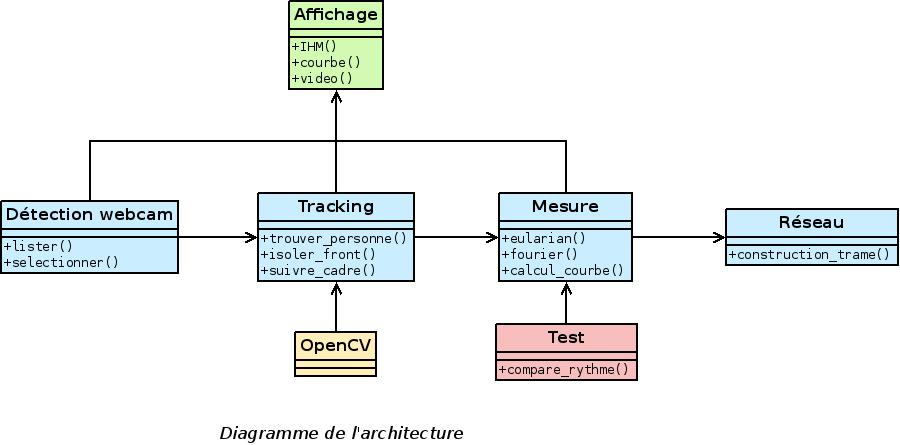
\includegraphics[scale=0.75,angle=90]{archi.jpeg}
\begin{center}

\end{center}

\includegraphics[scale=0.5]{bleu.png} : Modules implémentant besoins fonctionnels\newline

\includegraphics[scale=0.5]{vert.png} : Module d'affichage graphique\newline

\includegraphics[scale=0.5]{orange.png} : Framework\newline

\includegraphics[scale=0.5]{rouge.png} : Module de Test qui comprend un capteur arduino.\newline

\end{document}